%%% Dashboard Implementation
%%%%%%% Wording: ✅
%%%%%%% Styling: ✅
%%%%%%% References: ✅
%%%%% Grammar: ✅
%%% --------------------------------------------------------------
\chapter{Dashboard Implementation}
\label{ch:dashboard-implementation}

This chapter describes the implementation of a prototype analytical dashboard that visualizes the key findings from the analysis.
Using Dash and Plotly\footnote{Dash is a Python web application framework that enables the creation of interactive web applications using Plotly visualizations\cite{plotly_dash_plotly_com}.},
we developed a local development prototype that demonstrates how the analytical insights could be presented in an interactive format.
The implementation focused on efficient data querying, caching strategies for development, and handling asynchronous operations in Python.

The chapter details the technical approach, the challenges encountered during implementation (particularly with callback caching and async handling), and our solutions to these challenges.
While not intended for production deployment, the prototype successfully demonstrates the potential of the analytical findings in an interactive format.

%%% Section: Development Approach
%%% --------------------------------------------------------------
\begin{section}{Development Approach}
	\label{sec:implementation-development-approach}

	The implementation phase focused on transforming the analysis results from the~\autoref{ch:data-analysis-and-results} into an interactive dashboard prototype.
	Our approach prioritized rapid development and effective visualization of the analytical findings.

	Before proceeding with the development process, a considerable amount of time was spent on researching and testing different approaches in parallel to the data exploration and analysis.
	Several iterations were made to find the most development approach that would best fit the project's needs.

	\begin{subsection}{Development Goals}
		\label{subsec:implementation-development-approach-goals}

		The primary goal was to create a functional prototype dashboard that could effectively present the analysis results in an interactive format.
		The specific goals included demonstrating key findings through interactive visualizations, implementing basic filtering capabilities for data exploration,
		creating a responsive interface that handles data operations efficiently, and establishing a foundation for visualizing festival transaction data.
	\end{subsection}

	\begin{subsection}{Technology Selection}
		\label{subsec:implementation-development-approach-technology}

		The dashboard was built using Dash and Plotly, chosen primarily for their familiarity from prior personal experience.

		The technology stack included:
		\begin{itemize}
			\item Dash~\&~Plotly\footnote{\url{https://dash.plotly.com/}} using Python for the core dashboard framework
			\item Dash Mantine Components\footnote{\url{https://www.dash-mantine-components.com}} for enhanced UI elements
			\item PostgreSQL\footnote{\url{https://www.postgresql.org/}} for local data storage
		\end{itemize}

		This stack was chosen specifically for prototyping, with Dash and Plotly providing a good balance of functionality
		and development speed\cite{plotly_dash_plotly_com} based on previous personal experience using these tools in university projects.
		Mantine Components were added to enhance the visual presentation without significantly increasing additional development time.
	\end{subsection}

	\begin{subsection}{Local Development Focus}
		\label{subsec:implementation-development-approach-local}

		The dashboard was developed exclusively for the local environment, focusing on demonstrating analytical capabilities rather than production readiness.

		\vspace*{\fill}\pagebreak[4] % fill rest due to the foonote placement

		This decision was influenced by several factors:
		\begin{itemize}
			\item The prototype nature of the implementation, focusing on demonstrating analytical insights rather than production features.
			\item Complexity of Python async handling, production requirements, and deployment challenges with Python environments.
			\item Implementing a fully featured production-ready dashboard would require significant additional development time and would not bring additional value to the project.
		\end{itemize}

		Moreover, as stated previously, the personal motivation for this thesis was to learn more about the data and demonstrate the findings in an interactive way, leading to more insights and knowledge for future updates of the NFCtron Hub dashboard.

	\end{subsection}
\end{section}

%%% Section: Core Architecture
%%% --------------------------------------------------------------
\begin{section}{Core Architecture}
	\label{sec:implementation-core-architecture}

	Since it was developed for local use only, it did not require any complex environmental setups for the app nor the database.
	This significantly simplified and sped up the development process, allowing us to focus on the core functionality and visual presentation of the dashboard.

	The dashboard's architecture was designed to efficiently manage data during development, with a strong emphasis on query management and caching strategies.

	\begin{subsection}{Query Management System}
		\label{subsec:implementation-core-architecture-query-management}
		For the SQL database connection and pooling, the \texttt{asyncpg} library\footnote{\url{https://magicstack.github.io/asyncpg/current/}} was used,
		which provided a simple and efficient way to interact with the PostgreSQL database asynchronously using asyncio.

		To manage the SQL database interactions efficiently, a simple \textbf{Query Management System} has been implemented to handle loading data from our SQL database.

		It consisted of several key components:
		\begin{itemize}
			\item \textbf{QueryDefinition}: Defines query structure and parameters
			\item \textbf{QueryRegistry}: Maintains registered queries
			\item \textbf{QueryManager}: Handles query execution and caching
			\item \textbf{QueryParameter}: Defines parameter types and validation
		\end{itemize}

		The following example in~\autoref{lst:dashboard-implementation-query-management} demonstrates the query registration process:

		\begin{listing}[H]
			\caption{Query Management Example}
			\begin{minted}[breaklines]{python}
query_manager.registry.register_query(
    QueryDefinition(
        name="sankey_diagram",
        sql=QueryManager.process_sql_query("""
            SELECT * FROM get_sankey_diagram_data(:date_from$1, :date_to$2)
        """),
        parameters=[
            QueryParameter("date_from", datetime.datetime),
            QueryParameter("date_to", datetime.datetime)
        ],
        default_data="FSCacheDefault"  # Enables local CSV caching
    )
)
			\end{minted}
			\label{lst:dashboard-implementation-query-management}
		\end{listing}

		This class has been the core of the dashboard's data management, allowing multiple approaches to data loading and caching strategies.

		It allowed defining raw SQL queries with \texttt{QueryManager\.process\_sql\_query}, which safely handled parameter substitution and query formatting.
		Or it could have loaded an SQL query from an external file (due to the complexity of the query) and then executed it with parameters.

		On top of that, it allowed for defining default data loading strategies, such as loading data from a local CSV cache, which significantly sped up the development process.
		More of this is described in the following section.
	\end{subsection}

	\begin{subsection}{Dual Caching Strategy}
		\label{subsec:implementation-core-architecture-caching}

		To optimize the development process, the implementation uses two caching mechanisms that are complementary to one another.

		\begin{subsubsection}{Query Result Caching}
			\label{subsubsec:implementation-core-architecture-query-cache}

			Since the dashboard relies on several complex SQL queries to load data, it was crucial to optimize query execution.
			Running these queries repeatedly during development significantly slowed down the process.

			Thus, a basic file-based caching system was implemented to store query results as CSV files, preventing redundant database queries during the development.
			It, simply by defining a \texttt{default\_data} parameter in the \texttt{QueryDefinition} class, allowed turning on the caching for specific queries which did not need to be reloaded every time.

			The query execution handler shown in the~\autoref{lst:dashboard-implementation-query-cache} below
			\footnote{The implementation is rather a simplified pseudo-implementation, as the \texttt{execute\_query} method is more complex and contains additional logic for results formatting, database connection retries and error handling},
			demonstrates the simple implementation of this caching strategy.

			\begin{listing}[h]
				\caption{Query Result Caching Implementation}
				\begin{minted}[breaklines]{python}
def execute_query(self, query_name: str, parameters: Dict[str, Any], or_query_def: Optional[QueryDefinition]):
    query_key = self.get_query_key(query_name, parameters)

	# Load query from cache if enabled
    if query_def.default_data == "FSCacheDefault":
        try:
            return pd._read_csv_cache(query_key)
        except Exception as e:
            print(f"Failed to load query {query_name} from cache: {e}")

    # Execute database query directly
    result = self._execute_db_query(query_def, parameters)

    # Cache result for future use
    try:
        self._save_csv_cache(query_key, result)
    except Exception as e:
        print(f"Failed to save query {query_name} to cache: {e}")

    return result
				\end{minted}
				\label{lst:dashboard-implementation-query-cache}
			\end{listing}

			It firstly generates a unique query key based on the query name and its parameters in a form of hash, which then later was used as a directory and file path to the cached CSV data.

			Then, if the caching is enabled for the query, it tries to read the CSV file from the cache directory and return it as a result.
			Otherwise, it executes the DB query directly as usual and then saves the result to the cache directory for future use.
		\end{subsubsection}

		\vspace*{\fill}\pagebreak[4] % fill rest due to the foonote placement

		\begin{subsubsection}{Background Callback Caching}
			\label{subsubsec:implementation-core-architecture-callback-cache}

			Since the dashboard, when not using cached data, relied on long-running data processing operations, it was crucial to use Dash's background callbacks feature.
			These background callbacks run in a separate background process in a queue,
			allowing the main Dash application to remain responsive while the callback processes the data and then returns the result to the main application\cite{plotly_dash_plotly_com_background_callbacks}.

			Dash provides two options for background callback backends:

			\textbf{DiskCache}: Runs the callback logic in a separate process and stores the results to disk using the diskcache library.
			This is the easiest backend to use for local development but is not recommended for production.

			\textbf{Celery}: Runs the callback logic in a Celery worker\cite{celery_userguide_workers} and returns results to the Dash app through a Celery broker like Redis.
			This is recommended for production as it queues the background callbacks, running them one-by-one in the order that they were received by dedicated Celery worker(s).

			For our development, we used the DiskCache backend, as it was easier to set up and use for local development:

			\begin{listing}[H]
				\caption{DiskCache Background Callback Manager Setup}
				\begin{minted}[breaklines]{python}
CACHE_DIR = os.path.join(os.path.dirname(__file__), 'dash_cache')
os.makedirs(CACHE_DIR, exist_ok=True)
# cache configuration
cache = diskcache.Cache(
	directory=CACHE_DIR,
	size_limit=3e9,
	eviction_policy='least-recently-used',
)

# unique launch_uid to refresh cache when the app restarts
launch_uid = uuid4()
background_callback_manager = dash.DiskcacheManager(
	cache,
	cache_by=[lambda: launch_uid],
	expire=300
)
				\end{minted}
				\label{lst:dashboard-implementation-callback-cache}
			\end{listing}

			This implementation evolved through several iterations as we encountered scaling challenges.
			More on this is later described in the~\autoref{sec:implementation-technical-challenges}.
		\end{subsubsection}
	\end{subsection}

	\begin{subsection}{Custom Callback Management System}
		\label{subsec:implementation-core-architecture-callbacks}

		While developing the dashboard, we encountered a mismatch between our preferred asynchronous programming patterns and Dash's synchronous callback system.

		Having extensive experience with asynchronous programming in the JavaScript ecosystem, we wanted to leverage similar patterns in our Python implementation.
		This led to a custom callback management system implementation that somehow bridged this gap.

		The implementation addressed several development needs:
		\begin{itemize}
			\item \textbf{Async/Await Pattern Support}: The system allowed using familiar async/await syntax in our Python callbacks, maintaining consistency with the query execution manager, which was already implemented using async
			patterns.
			\item \textbf{Unified Error Handling}: Instead of implementing error handling in each callback separately, the decorator provided centralized, but simple, error management and logging, reducing code duplication and ensuring
			consistent error handling across all callbacks.
			\item \textbf{Flexible Processing Modes}: The system seamlessly supported both synchronous and asynchronous operations through a single interface, automatically managing asyncio event loops
			\footnote{Asyncio is a Python library to write concurrent code using the async/await syntax\cite{psf_library_asyncio}} when needed.
		\end{itemize}

		The simplified pseudo-implementation
		\footnote{
			The actual implementation includes additional features such as proper asyncio event loop management, argument parsing, and integration with the caching system.
			This example demonstrates the core pattern while omitting implementation details.}, shown in~\autoref{lst:dashboard-implementation-callback-decorator}, demonstrates this approach to the custom callback registration.

		\begin{listing}[H]
			\caption{Custom Callback Decorator Implementation}
			\begin{minted}[breaklines]{python}
def register_callback(self, output, inputs, background=False):
	def decorator(func):
		async def async_wrapper(_self, *args):
			try:
				return await func(_self, *args)
			except Exception as e:
				print(f"Error in {func.__name__}: {str(e)}")
				raise dash.exceptions.PreventUpdate

		if background:
			return self.__app.callback(
				output=output,
				inputs=inputs,
				background=True,
				*args, **kwargs
			)(async_wrapper)
		return self.__app.callback(output=output, inputs=inputs, *args, **kwargs)(func)

	return decorator
			\end{minted}
			\label{lst:dashboard-implementation-callback-decorator}
		\end{listing}

		This unified approach simplified the possibly complex and boiler-plated, callback implementations, as shown in~\autoref{lst:dashboard-implementation-callback-usage}:

		\begin{listing}[H]
			\caption{Callback Registration Example}
			\begin{minted}[breaklines]{python}
@register_callback(
    output=Output("sankey-diagram", "figure"),
    inputs=[
        Input("date-range", "start_date"),
        Input("date-range", "end_date")
    ],
    background=True
)
async def update_sankey_diagram(self, start_date, end_date):
    data = await self.query_manager.execute_async(
        "sankey_diagram",
        parameters={"date_from": start_date, "date_to": end_date}
    )
    return create_sankey_figure(data)
			\end{minted}
			\label{lst:dashboard-implementation-callback-usage}
		\end{listing}

		This method worked seamlessly with the query management system and offered flexibility for simple and complex data processing.
		The combination of background processing and proper error handling proved essential for managing the complex data flows in the dashboard.

		It allowed a better focus on callback business logic because the decorator pattern encapsulated the complexity of bridging sync and async environments.
	\end{subsection}

	\begin{subsection}{Dashboard Structure}
		\label{subsec:implementation-core-architecture-structure}

		The dashboard has been structured to reflect the analysis sections from the~\autoref{ch:data-analysis-and-results}, with dedicated sections for:
		\begin{itemize}
			\item \textbf{Cashflow and Revenue Analysis},
			\item \textbf{Performance Analysis},
			\item \textbf{Beverage Consumption Analysis},
			\item and \textbf{Customer Analysis}.
		\end{itemize}

		Each section implements background callbacks for data loading and filtering, using the dual caching strategy to maintain responsiveness during development.

		For each section, a separate file was created, containing the layout and callback definitions for the section.
		The main dashboard file then imports these sections and combines them into a single layout.

		This approach allowed for better code organization and easier development of individual sections.
	\end{subsection}
\end{section}

%%% Section: Technical Challenges and Solutions
%%% --------------------------------------------------------------
\begin{section}{Technical Challenges and Solutions}
	\label{sec:implementation-technical-challenges}

	The implementation process encountered several significant technical challenges, primarily centered around asynchronous operations and callback caching in Python.
	These challenges and their solutions significantly influenced the overall development approach and the outcome of the dashboard prototype.

	\begin{subsection}{Asynchronous Handling Challenges}
		\label{subsec:implementation-technical-challenges-async}

		Coming from a JavaScript background, where asynchronous programming is relatively straightforward\cite{node.js_asynchronous_work_javascript_asynchronous_programming_and_callbacks}, Python's async implementation presented several challenges.
		The main difficulties arose in implementing background tasks for the dashboard's filtering capabilities and data loading operations whilst already having implemented the query management system using async patterns.

		However, thanks to the~\fullref{subsec:implementation-core-architecture-callbacks} implementation, it was possible to leverage Python's async/await patterns effectively.
	\end{subsection}

	\begin{subsection}{Callback Caching Evolution}
		\label{subsec:implementation-technical-challenges-caching}

		The evolution of the callback caching solution went through several iterations, each addressing specific challenges, as described below.

		\begin{subsubsection}{Initial Implementation}
			\label{subsubsec:implementation-technical-challenges-caching-initial}

			Following Dash documentation\cite{plotly_dash_plotly_com_background_callbacks}, we initially implemented a single \texttt{DiskcacheManager} with a simple cache directory setup:

			\begin{listing}[H]
				\caption{Initial Cache Manager Setup}
				\begin{minted}[breaklines]{python}
cache = diskcache.Cache(directory=CACHE_DIR)
background_callback_manager = dash.DiskcacheManager(
    cache,
    expire=300
)
				\end{minted}
				\label{lst:dashboard-implementation-cache-initial}
			\end{listing}

			However, since our dashboard had several callbacks registered, and many had the same inputs,
			due to the modular structure of the dashboard\footnote{Each dashboard section had its own callbacks; but many of them shared the same inputs, such as date range filters}, this approach led to cache key collisions.

			\begin{infobox}{Why Cache Key Collisions Occurred}
				\textbf{Cache Key Collisions} occurred because the~\textt{DiskcacheManager} used the same cache key for callbacks with identical inputs.
				We did not know that the callbacks should ideally have unique inputs to prevent cache key collisions.
				As a result, the cached data was overwritten, leading to incorrect data being returned.
			\end{infobox}
		\end{subsubsection}

		\begin{subsubsection}{First Solution Attempt}
			\label{subsubsec:implementation-technical-challenges-caching-first}

			To address cache key collisions, we tried to implement a unique~\textt{DiskcacheManager} instance for each unique callback, based on it's~\texttt{callback\_id}:

			\begin{listing}[H]
				\caption{Unique Cache Managers Per Callback}
				\begin{minted}[breaklines]{python}
def create_callback_manager(callback_id):
    return dash.DiskcacheManager(
        cache,
        cache_by=[
            lambda: launch_uid,
            lambda: callback_id
        ]
    )
				\end{minted}
				\label{lst:dashboard-implementation-cache-unique}
			\end{listing}

			This solution worked well for individual dashboard sections but revealed issues when scaling and combining all dashboard sections together.
		\end{subsubsection}

		\begin{subsubsection}{Scaling Challenges}
			\label{subsubsec:implementation-technical-challenges-caching-scaling}

			As the number of callbacks increased, we encountered SQLite concurrent connection issues.
			The local SQLite database used by DiskcacheManager\footnote{\url{https://grantjenks.com/docs/diskcache/}} could not handle multiple concurrent write connections effectively, causing the dashboard to crash during loading.
			It was caused because each callback had its own DiskcacheManager instance, which created a separate SQLite connection for each callback, and all of them were trying to write to the same SQLite database file.

			A more robust solution, recommended for production setup in Dash documentation – Celery~\&~Redis
			\footnote{Celery is a distributed task queue that allows for background task execution, while Redis is an in-memory data structure store used as a database, cache, and message broker\cite{reintech_blog_combining_celery_redis_caching_task_queuing}\cite{celery_getting_started_introduction}\cite{redis_latest}},
			was considered as a solution to this issue.

			Such a solution looked promising since it would allow for each callback to define \texttt{cache\_by} parameter.
			This would be unique for each callback, and then the Celery worker would process the tasks in the order they were received, effectively preventing concurrent SQLite connection issues.

			Due to the complexity of the setup, especially the Celery, and relatively a lack of instructions and functional examples, it was not easy to make it work in the local development environment.

			We successfully set up the Redis server and Celery worker, but the integration with Dash was not successful.
			The Celery worker was not registering the tasks from the Dash app, despite following all available guides and examples.
			This resulted in no tasks being processed by the Celery worker, and the dashboard was not able to load any data.

			Eventually, after an unsuccessful 12–hour overnight journey, we decided to look for a simpler solution as a result of the frustration, lack of progress, and time constraints.

			Then a simple and dumb, yet effective solution was found, which was to create a separate cache directory for each callback,
			effectively isolating the SQLite database for each callback, as shown in the~\autoref{lst:dashboard-implementation-cache-final}.

			\vspace*{\fill}\pagebreak[4] % fill rest due to the foonote placement

			\begin{listing}[H]
				\caption{Final Cache Implementation}
				\begin{minted}[breaklines]{python}
def create_isolated_cache_manager(callback_id):
    # Create separate cache database per callback
    cache_dir = os.path.join(os.path.dirname(__file__), f'dash_cache_{callback_id}')
    cache = diskcache.Cache(directory=cache_dir)

    return dash.DiskcacheManager(
        cache,
        cache_by=[
            lambda: launch_uid,
            lambda: callback_id
        ],
        expire=300
    )
				\end{minted}
				\label{lst:dashboard-implementation-cache-final}
			\end{listing}

			While this solution is not production-ready and nearly on the edge of being a hack, it effectively solved the local development needs and allowed us to continue development without further issues.
		\end{subsubsection}
	\end{subsection}
\end{section}

%%% Section: Implementation Results
%%% --------------------------------------------------------------
\begin{section}{Implementation Results}
	\label{sec:implementation-results}

	The dashboard prototype successfully demonstrates key findings from our festival analysis through interactive visualizations.
	Drawing from our analytical framework, we organized the interface into four main sections that provide different perspectives on the event data.

	A global date-range filter, shown in the~\autoref{fig:dashboard-header}, sits at the top of the dashboard, allowing users to analyze any time period during the festival.
	Pre-configured options for each festival day make it easy to quickly compare different phases of the event.

	\begin{figure}[H]
		\centering
		
\includegraphics[width=\textwidth]{\ThesisFigures/ui/dashboard-header}
		\caption{Dashboard Header with Date Range Filter}
		\label{fig:dashboard-header}
		\source
	\end{figure}

	\begin{subsection}{Cashflow and Revenue Analysis Section}
		\label{subsec:implementation-results-structure-cashflow}

		The financial section gives an immediate overview of money flows through the festival system.
		Three key metrics at the top show the total revenue (\bfmtczk{1155162}), available balances (\bfmtczk{334450}), and total chip top-ups (\bfmtczk{14520973}).
		A visual representation of this section is shown in~\autoref{fig:dashboard-cashflow-analysis}.

		\begin{figure}[h]
			\centering
			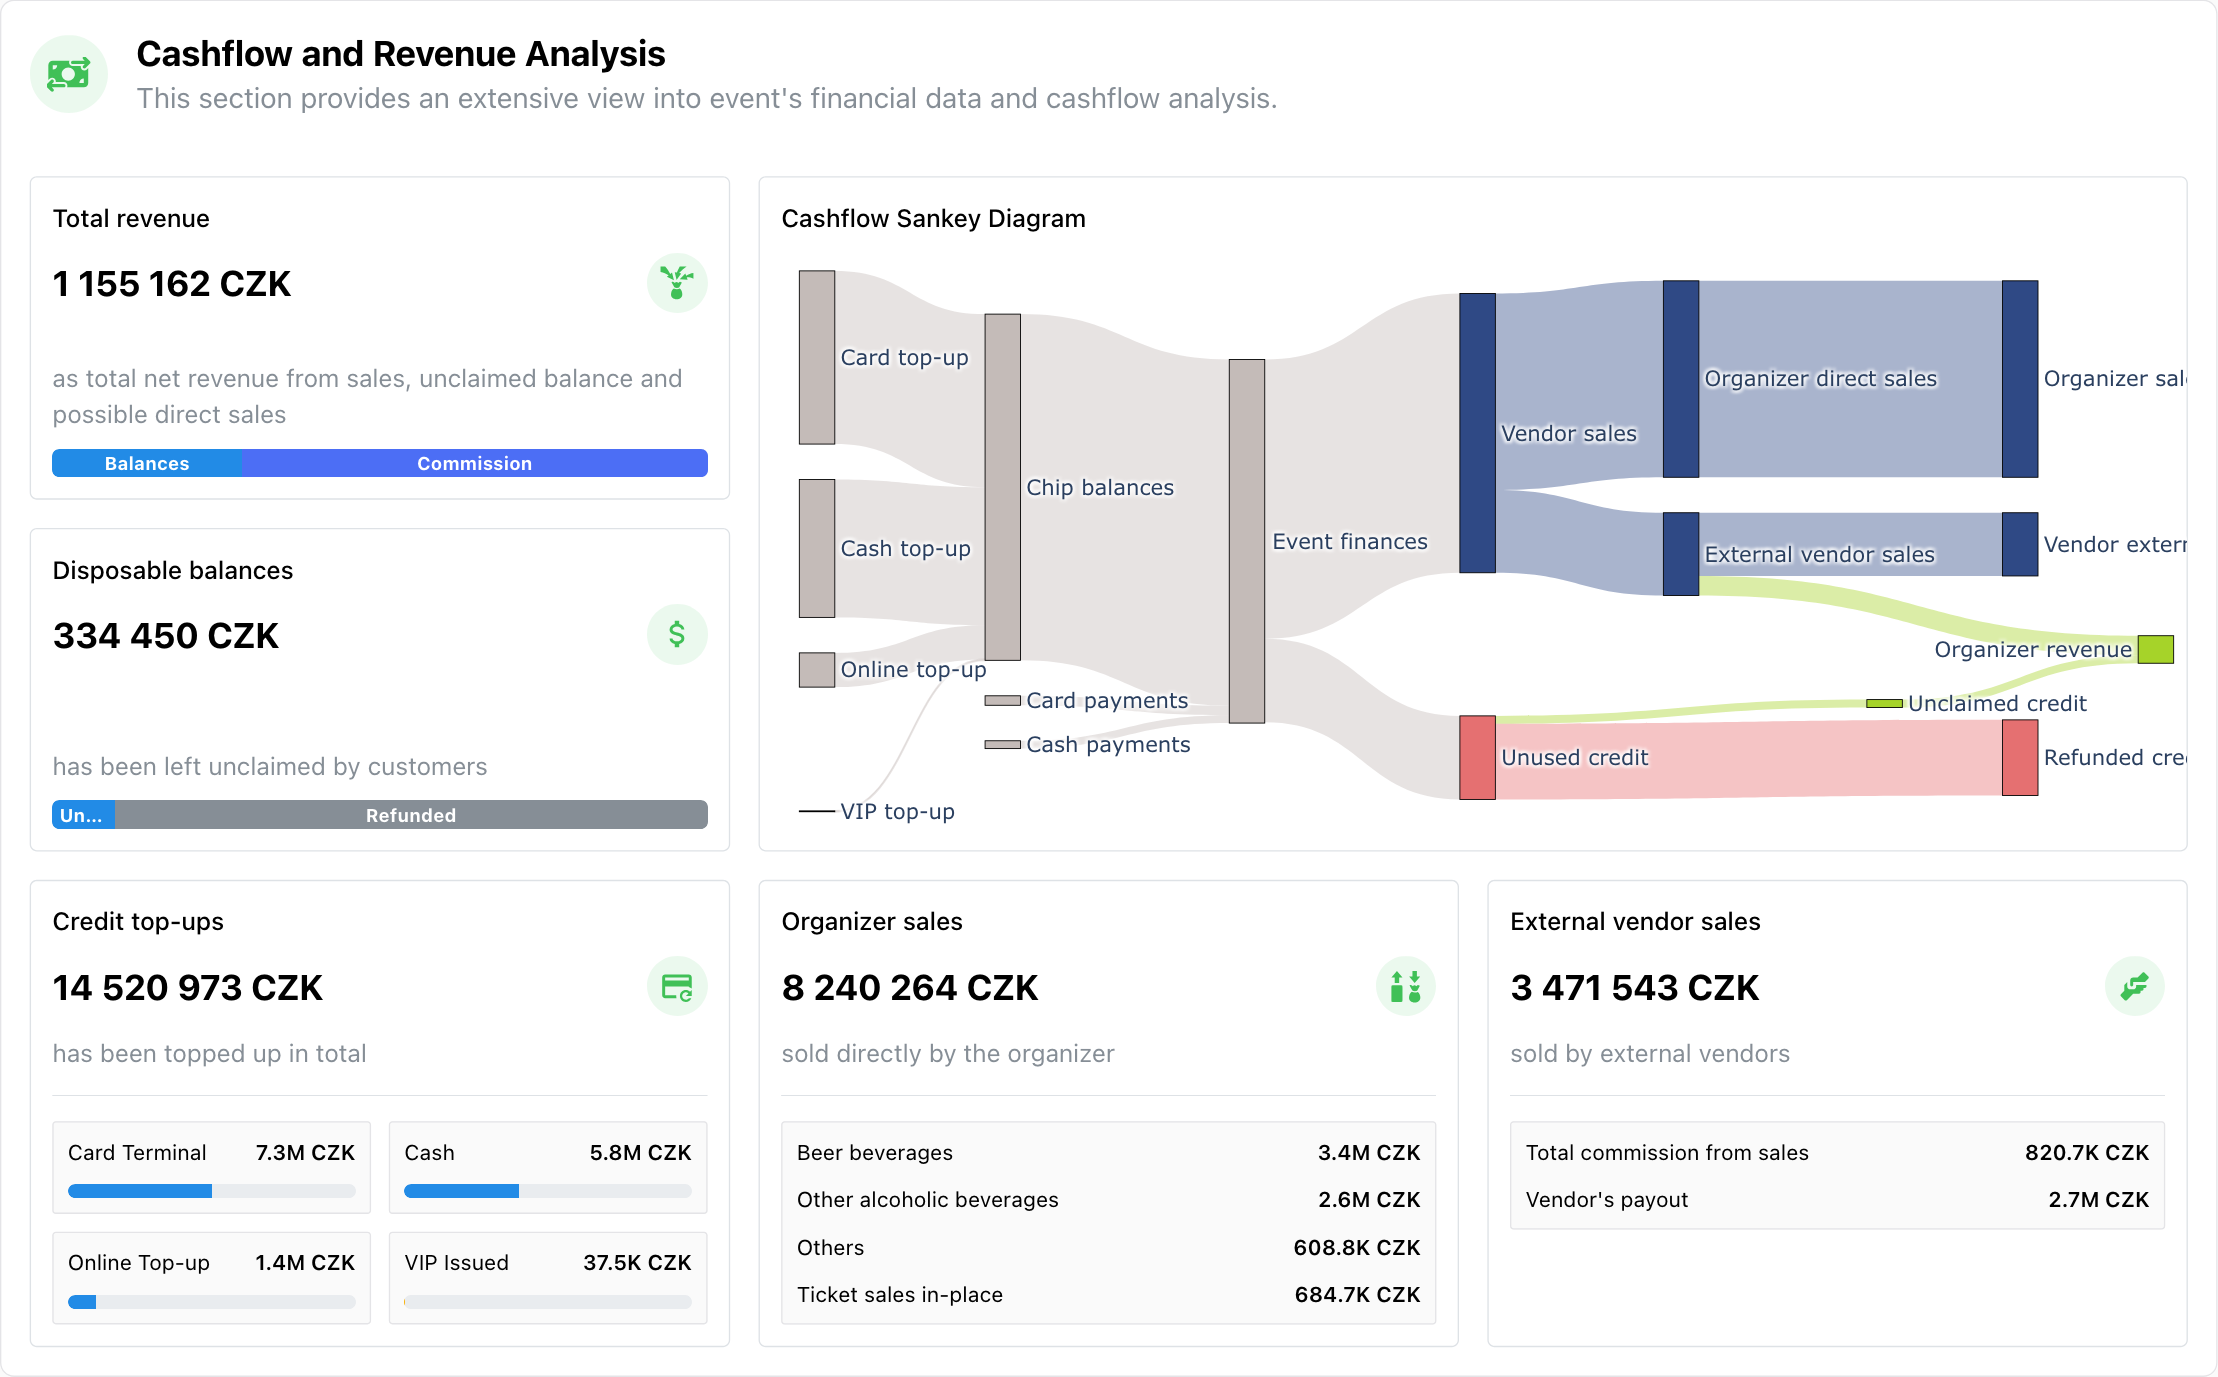
\includegraphics[width=\textwidth]{\ThesisFigures/ui/dashboard-cashflow-section}
			\caption{Cashflow and Revenue Analysis Section}
			\source
			\label{fig:dashboard-cashflow-analysis}
		\end{figure}

		The centerpiece Sankey diagram visualizes how money moves through the system—from initial top-ups through various payment channels to final settlements.
		This helps to track the conversion of chip credits into sales and monitor refund volumes.

		Below, the data splits between organizer sales (\bfmtczk{8240264}) and external vendor sales (\bfmtczk{3471543}), with detailed breakdowns for beverages, food, and other related information.
	\end{subsection}

	\begin{subsection}{Performance Analysis Section}
		\label{subsec:implementation-results-structure-performance}

		The performance section helps to understand operational dynamics throughout the festival.
		Key metrics prominently display the festival's scale: \bfmtnum{10009}~active customers, \bfmtnum{141378}~processed transactions, and a peak volume of~\bfmtnum{8986}~transactions per hour.
		A visual representation of this section is shown in~\autoref{fig:dashboard-performance-analysis}.

		\begin{figure}[h]
			\centering
			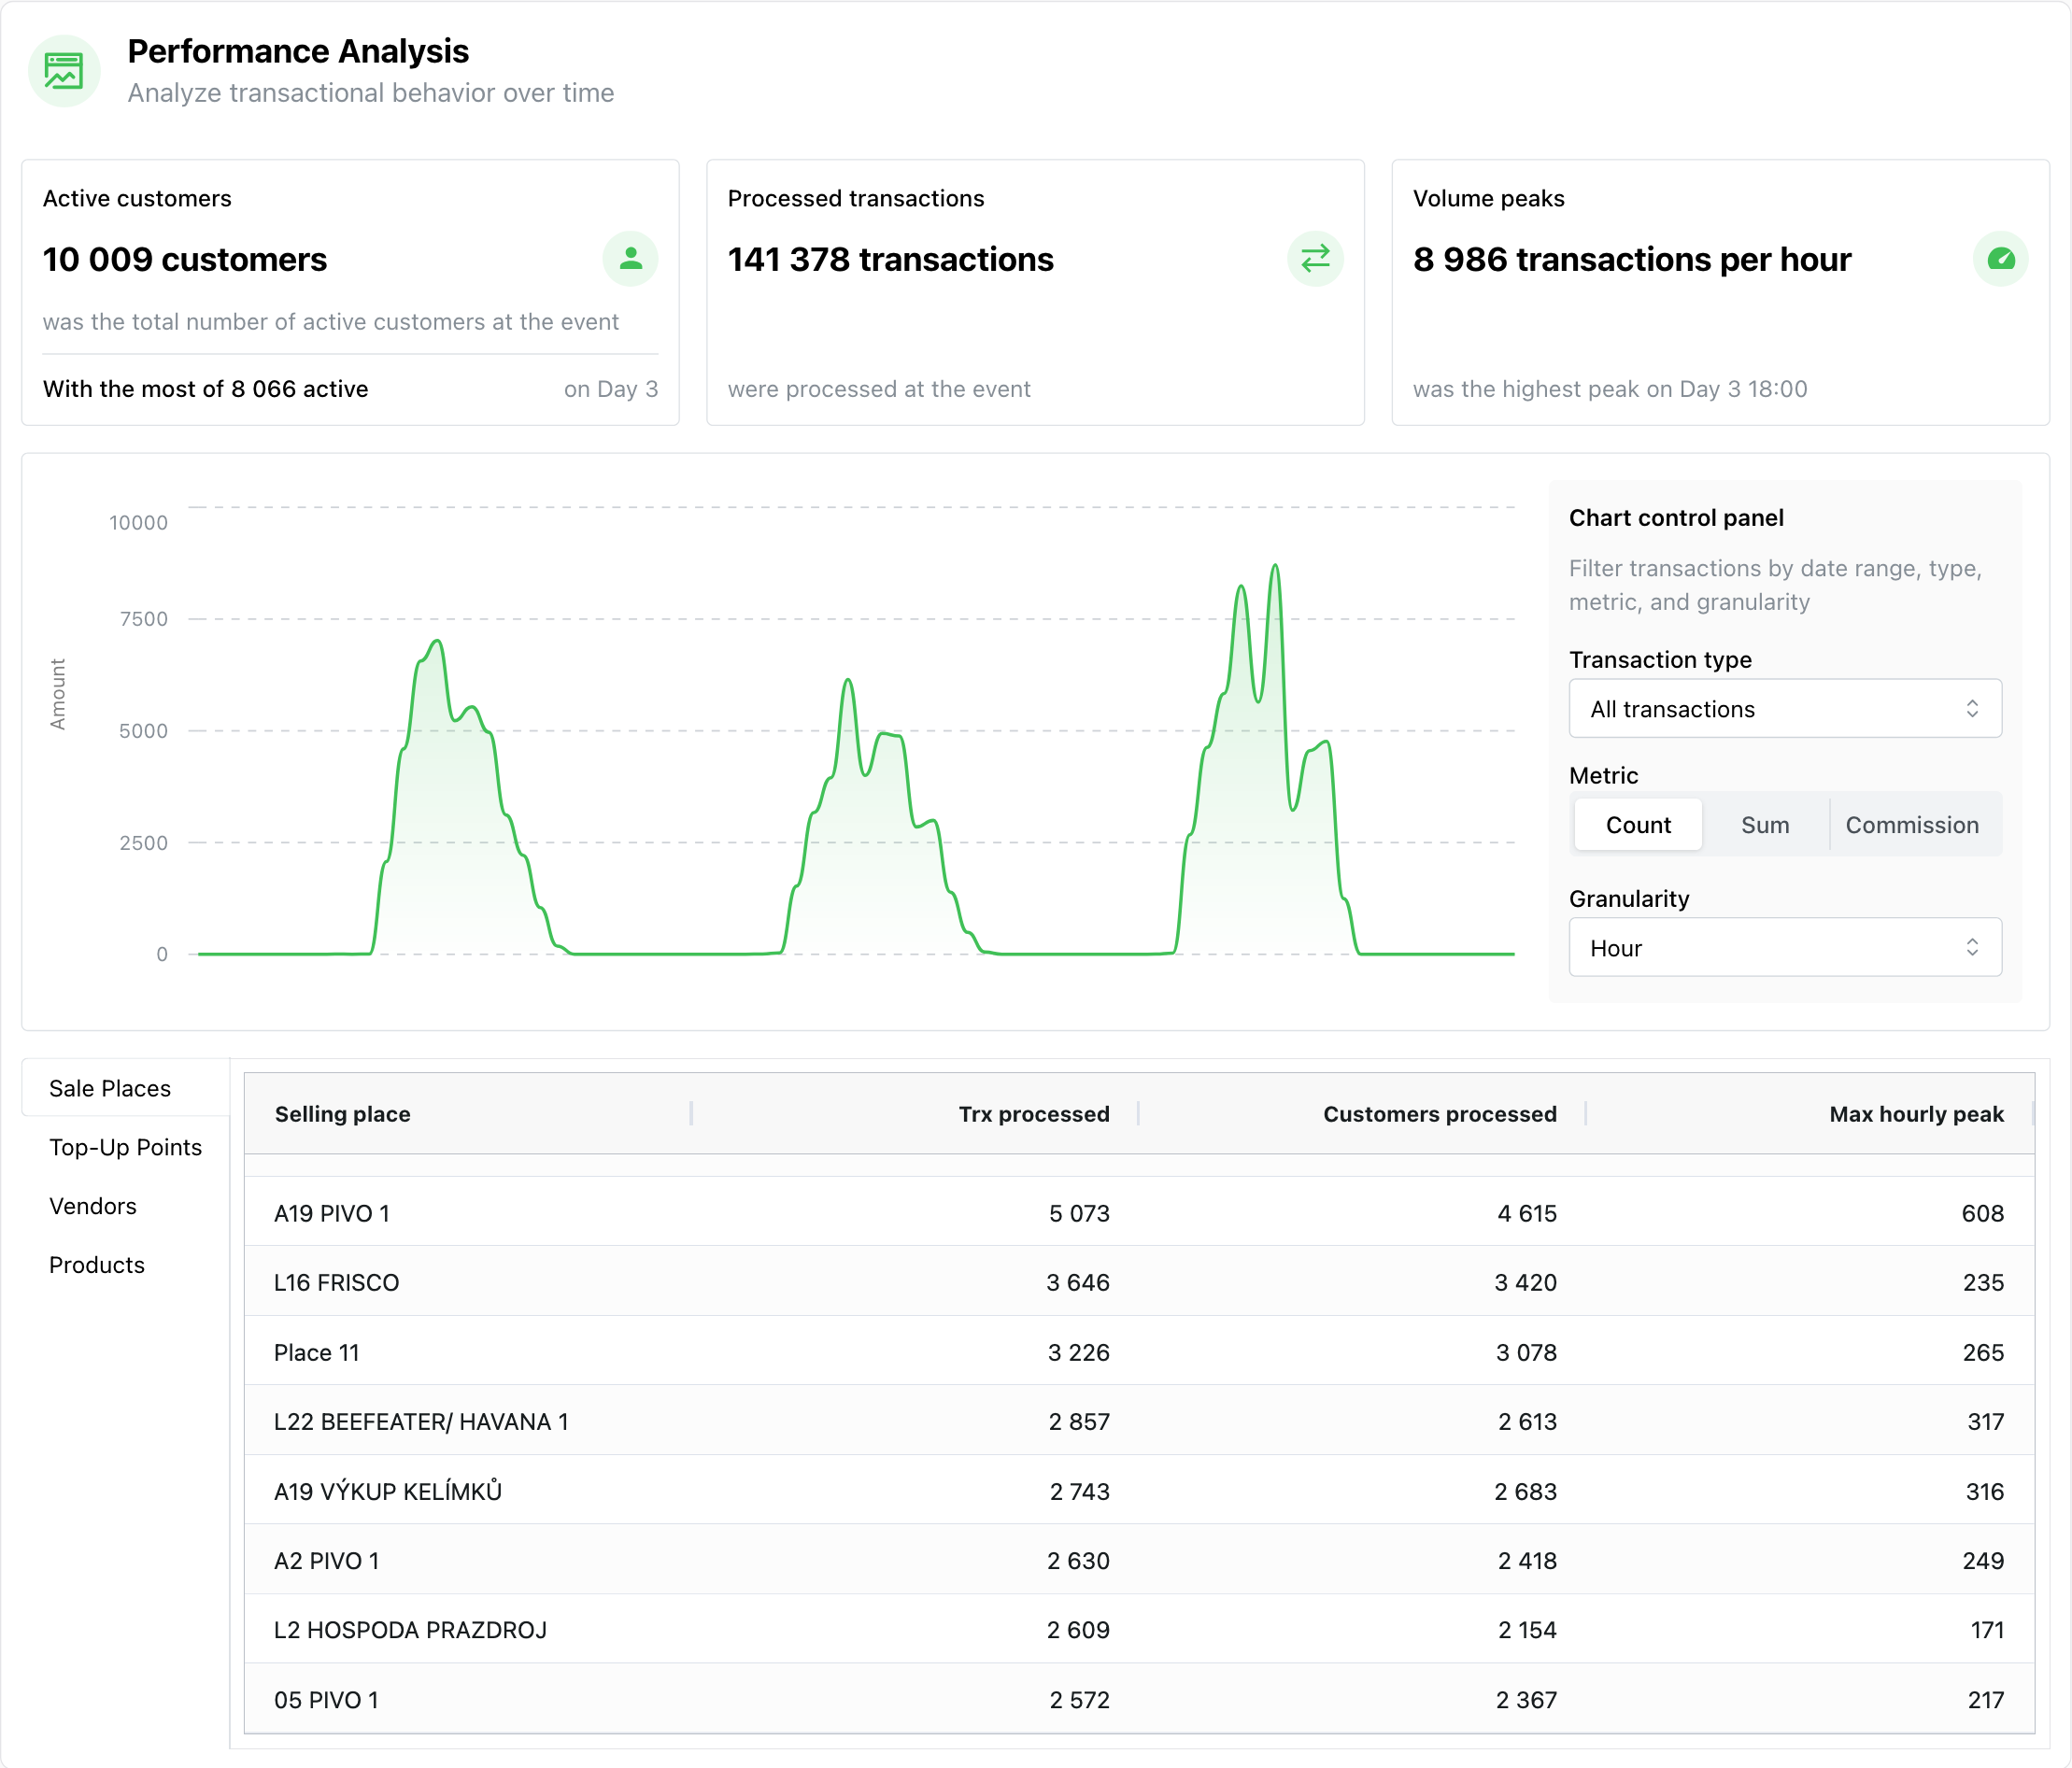
\includegraphics[width=\textwidth]{\ThesisFigures/ui/dashboard-performance-section}
			\caption{Performance Analysis Section}
			\source
			\label{fig:dashboard-performance-analysis}
		\end{figure}

		The main graph shows transaction volumes across all three days, with the highest peak visible on Day~3 at~18:00.

		The control panel can be used to filter by transaction types and adjust time granularity for detailed analysis.

		A table below highlights the busiest operational points, showing how many transactions and customers each location handled, as well as for individual vendors or products.
	\end{subsection}

	\begin{subsection}{Beverage Consumption Analysis Section}
		\label{subsec:implementation-results-structure-beverage}

		The beverage section tracks consumption patterns and returnable cup management.
		At a glance, a total consumption (\bfmtnum{35844}~liters), returnable cups issued (\bfmtnum{22045}), and the return rate of~\bfmtnump[2]{78.4}\% can immediately be seen.
		A visual representation of this section is shown in~\autoref{fig:dashboard-beverage-analysis}.

		\begin{figure}[h]
			\centering
			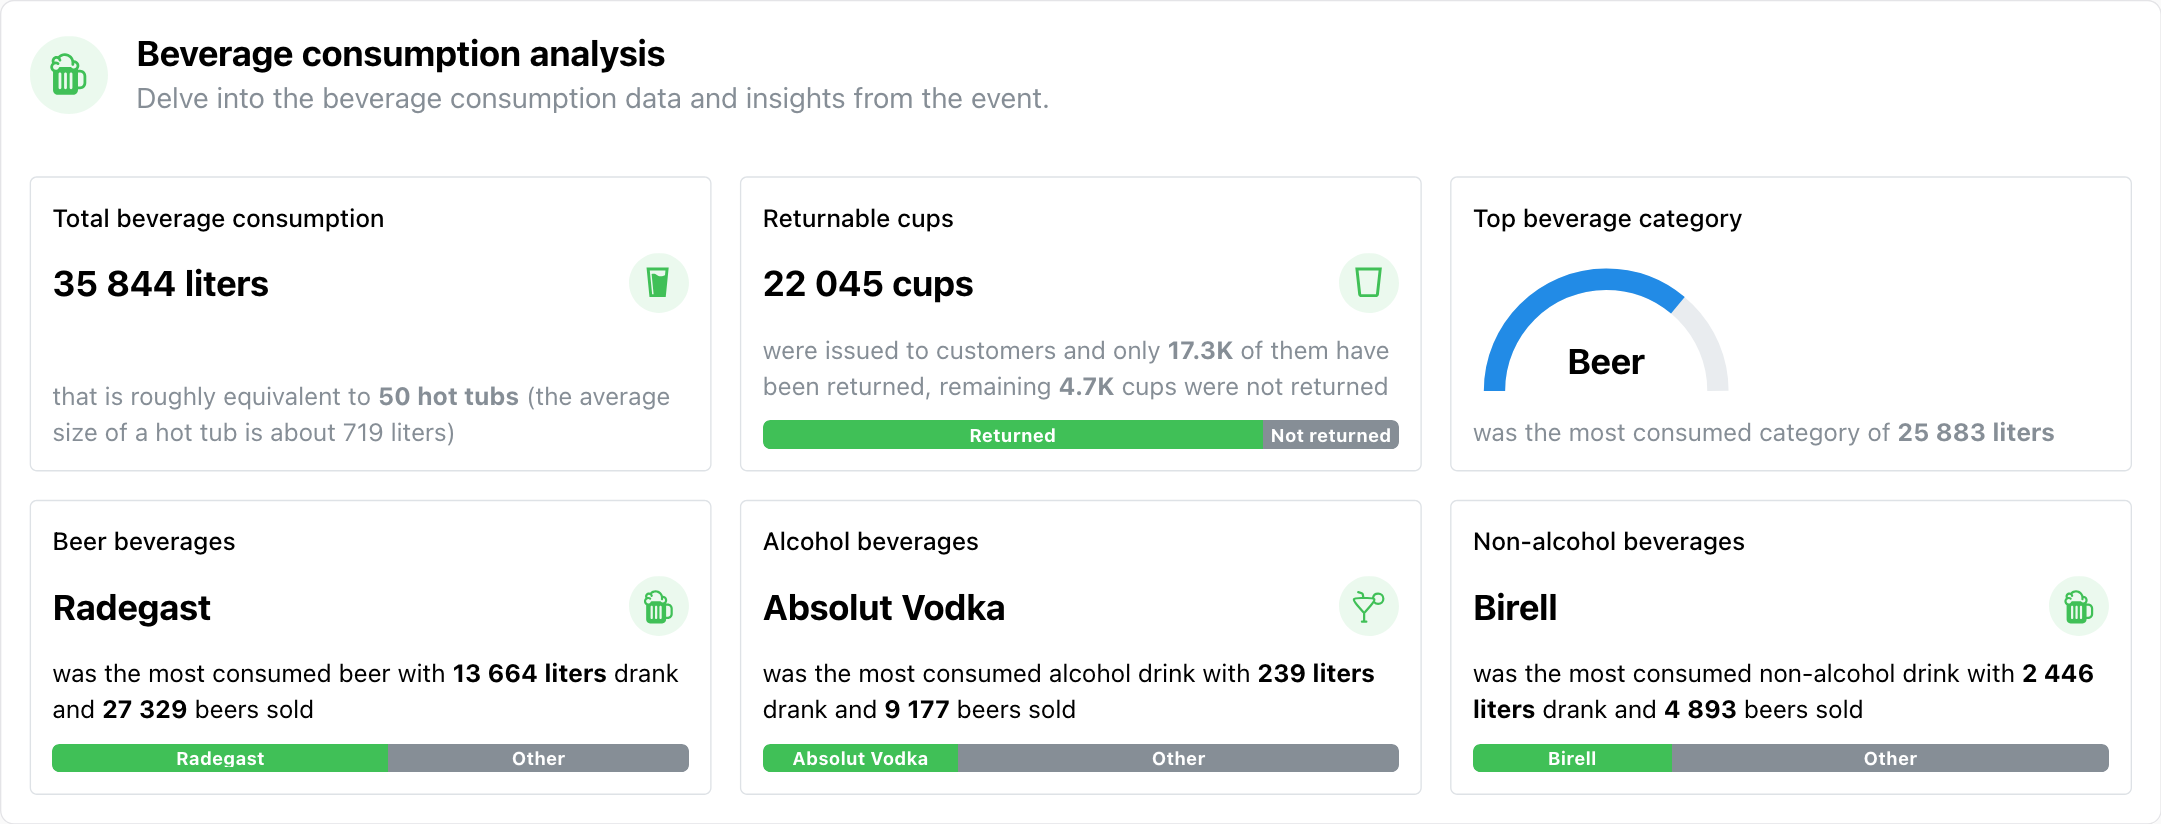
\includegraphics[width=\textwidth]{\ThesisFigures/ui/dashboard-beverage-section}
			\caption{Beverage Consumption Analysis Section}
			\source
			\label{fig:dashboard-beverage-analysis}
		\end{figure}

		Breaking down by category, \textbf{Radegast} led beer sales with \bfmtnum{13665}~liters and \bfmtnum{27329}~units sold.
		\textbf{Birell} dominated non-alcoholic beverages with \bfmtnum{2446}~liters, while \textbf{Absolut Vodka} led spirits with \bfmtnum{239}~liters consumed.
	\end{subsection}

	\begin{subsection}{Customer Analysis Section}
		\label{subsec:implementation-results-structure-customer}

		While currently still in development, the customer analysis section aims to provide insights into attendee behavior patterns.
		The planned implementation focuses on four key areas of visitor analysis.

%\begin{figure}[h]
%	\centering
%	
\includegraphics[width=\textwidth]{\ThesisFigures/ui/dashboard-customer-section}
%	\caption{Customer Analysis Section (Implementation in Progress)}
%	\source
%	\label{fig:dashboard-customer-analysis}
%\end{figure}

		The attendance timeline will show how \bfmtnum{10009}~unique visitors were distributed across the festival, with Day~3 seeing peak attendance of~\bfmtnum{8066}~visitors.
		Customer segmentation will break down the \bfmtnump[2]{89.66}\%~online ticket purchasers and track platform preferences, including the \bfmtnump[2]{40.69}\%~mobile app usage rate.
		Payment analysis will visualize card scheme preferences (VISA~\bfmtnump[2]{62.4}\%, Mastercard~\bfmtnump[2]{37.6}\%) and top-up patterns.

		This section represents a key area for future development, particularly for exploring customer behavior patterns.
		Unfortunately, due to the time constraints, it was not possible to finish the implementation of this section during the thesis project.
		However, the key findings from the analysis were already prepared and ready to be implemented.
	\end{subsection}
\end{section}


%%% Section: Missing Features and Future Development
%%% --------------------------------------------------------------
\begin{section}{Missing Features and Future Development}
	\label{sec:future-development}

	While the current implementation successfully demonstrates our analysis results, there are several directions for future development and improvement.

	\begin{subsection}{Technical Improvements}
		\label{subsec:future-technical}

		From a technical perspective, several key improvements would be needed for production deployment:

		\textbf{Infrastructure and Deployment}: The current implementation is limited to local setup with a local database.
		Significant architectural changes would be needed to enable external access and proper production deployment with a more robust database solution and data layer separation.

		\textbf{Performance Optimization}: SQL queries would require optimization for larger datasets.
		Implementation of materialized views and better query planning would improve response times with production-scale data.
		\footnote{Materialized views are essentially database tables that store the results of a query and can be used to improve query performance\cite{tpgdg_current_rules_materializedviews}}

		\textbf{Caching Solution}: A production-grade caching system using Redis would replace the current development-focused implementation.
		This would improve dashboard responsiveness and enable handling multiple concurrent users.

		\textbf{Data Formatting}: Enhanced date formatting and chart configurations would improve data presentation.
		The current implementation uses basic formatting which would need refinement for production use.
	\end{subsection}

	\begin{subsection}{Analytical Enhancements}
		\label{subsec:future-analytical}

		From an analytical perspective, several key features would enhance the dashboard's utility:

		\textbf{Customer Analysis}: Complete implementation of the customer analysis section would provide valuable insights into attendee behavior.
		This would enable better understanding of customer segments and their preferences.

		\textbf{Performance Metrics}: Expansion of the performance section with detailed time processing metrics would provide better operational insights.
		This would help identify bottlenecks and optimization opportunities.

		\textbf{Timeline Navigation}: A dynamic timeline player would allow users to observe festival data evolution over time.
		This would enable to replay the festival's progression and identify critical moments or patterns.

		\textbf{Interactive Elements}: Additional interactive features would allow users to switch between different metrics and apply more granular filters.
		This flexibility would help to discover deeper insights and test different hypotheses about festival operations.
	\end{subsection}
\end{section}


